\documentclass[12pt]{article}
\usepackage[paper=a4paper,left=30mm,right=30mm,top=35mm,bottom =35mm]{geometry}
\usepackage[utf8]{inputenc}
\usepackage[T1]{fontenc}
\usepackage{stmaryrd}
\usepackage{setspace}
\usepackage{mathrsfs}
\usepackage[ngerman]{babel}
\usepackage{amssymb}
\usepackage{amsmath}
\usepackage{fancyhdr}
\usepackage[dvips,unicode,colorlinks,linkcolor=black]{hyperref} 
\usepackage{graphicx}
\usepackage{float}

\pagestyle{fancy}
\lfoot{}
\rfoot{Paul Kremser, Tobias Grussenmeyer}
\cfoot{\thepage}
\fancyhead[L]{FPII Versuch: Mösbauereffekt}
\renewcommand{\headrulewidth}{0.6pt}
\renewcommand{\footrulewidth}{0.6pt}
\setlength{\headheight}{16pt}
\setlength{\parindent}{0pt}
% Für die Wahl der Schriftart
\newcommand{\changefont}[3]{
\fontfamily{#1} \fontseries{#2} \fontshape{#3} \selectfont}
%\renewcommand{\vec}[1]{\mathbf{#1}}
\renewcommand*\vec[1]{{\mbox{\boldmath\ensuremath{#1}}}}

\begin{document}
% keine Hurenkinder und Schusterjungen
\clubpenalty = 10000
\widowpenalty = 10000 
\displaywidowpenalty = 10000

\onehalfspacing
% Schriftart
\changefont{ptm}{m}{n} 

\begin{titlepage}
\author{Paul Kremser, Tobias Grussenmeyer}
\title{Versuch: Mösbauereffekt}
\date{Versuchsdurchführung: 1. bis 12. März 2010} 
\maketitle
\thispagestyle{empty}
\end{titlepage}


\tableofcontents
\thispagestyle{empty}
\newpage
\pagenumbering{arabic}
\section{Überblick}
Stichwort rückstoßfreie Resonanzabsorption: Emmitiert ein Kern Strahlung in Form eines Photons, so hat dieses Photon einen Impuls.
Nach der Impulserhaltung muss also auch der strahlende Kern gerade diesen Impuls in entgegengesetzter Richtung erhalten. Der Kern hat nach Aussendung des Photons eine Geschwindigkeit, folglich eine kinetische Energie. Dem Photon fehlt sozusagen genau die Energie welche der Kern für die Bewegung hat. Von 'Fehlen' spricht man, da die Energie des Photons nun nicht ausreicht um einen anderen (ruhenden) Kern anzuregen. Um die Anregung zu ermöglichen müsste dieser Kern sich mit der 'doppelten Geschwindigkeit' des ersten auf das Photon zu bewegen.

Bindet man die Kerne nun aber in Kristalle ein so muss der Impuls des Photons irgentwie auf den gesamten Kristall übergehen. Im glücklichten Fall entsteht hierbei kein Phonon im Kristall und die dem Photon fehlende Energie geht mit steigender Masse des Kristalls gegen Null. Man spricht von rückstoßfreier Resonanzabsorption, das Photon kann nun einen anderen Kern anregen.
\section{Aufgabestellung}
\begin{enumerate}
 \item Verkabelung des Aufbaus, Einstellungen der Elektronik (Verstärker, Delay, SCA und Gate).
 \item Energieeichung des MCA mit Hilfe eines Americium Strahlers und verschiedener metallischer Floureszenzplättchen (Aufbau mit Drehscheibe)
 \item Mit dem SCA ein Fenster auf die 14,4 KeV Linie setzen.
 \item Mit Hilfe verschiedener Aluminiumplättchen sollen Untergrundmessungen bei verschiedenen Dicken gemacht werden um später auf die Dicke Null extrapolieren zu können.
 \item Aufnahme der Spektren des Einlinien- (Eisen) absorbers und des 6-Linien- (Edelstahl) absorbers.
\end{enumerate}




\section{Theoretische Grundlagen}
Wie schon im Überblick erwähnt geht es beim Mößbauereffekt um das Auftreten rückstoßfreier Kernresonanzabsorption.
In unserem Fall wird der Mößbauereffekt an der 14,4keV-Linie von $^{57}Fe$ beobachtet. 

\subsection{Resonanzabsorption}
Geht ein Kern unter Aussendung eines Photons von einem angeregten Zustand $E_a$ in den Grundzustand $E_g$ über und regt dieses Photon
wiederum einen anderen Kern aus dem
Grundzustand $E_g$ in den selben angeregten Zustand $E_a$ an, so spricht man von Resonanzabsorption.

Ein freies ruhendes Atom bzw. ruhender Kern mit Masse $m$ erhält bei Emission eines Photons $\gamma$ aufgrund der Impulserhaltung
gerade den entgegengesetzten Impuls des ausgesendeten Photons:
\begin{align}
 \vec{p}_g = -\vec{p}_\gamma = \hbar\vec{k}
\end{align}
Für die Energie dieses Rückstoßes erhält man mit der Photonenenergie $E^2_\gamma = \vec{p}^2_\gamma c^2$:
\begin{align}
 E_R = \frac{\vec{p}_g^2}{2m} = \frac{\vec{p}^2_\gamma}{2m} = \frac{E^2_\gamma}{2mc^2}
 \label{e_r}
\end{align}
Die Energie des Übergangs $E = E_a - E_g$ teilt sich also auf die Rückstoßenergie und die Photonenenergie auf:
\begin{align}
 E = E_R + E_\gamma
\end{align}
Somit entspricht die Energie des emmitierten Photons nicht ganz der des Übergangs. Ebenso wird bei der Absorption eines Photons durch einen freien ruhenden
Kern ein Impuls auf den Kern übertragen. Insgesamt fehlt für die Resonanzabsorption bei freien ruhenden Atomen bzw Kernen also der Energiebetrag von $2E_R$.
Damit sind die Emissions- und Absorptionslinie gegeneinander Energieverschoben. (Siehe Abbildung. \ref{energieverschiebung})
\begin{figure}
 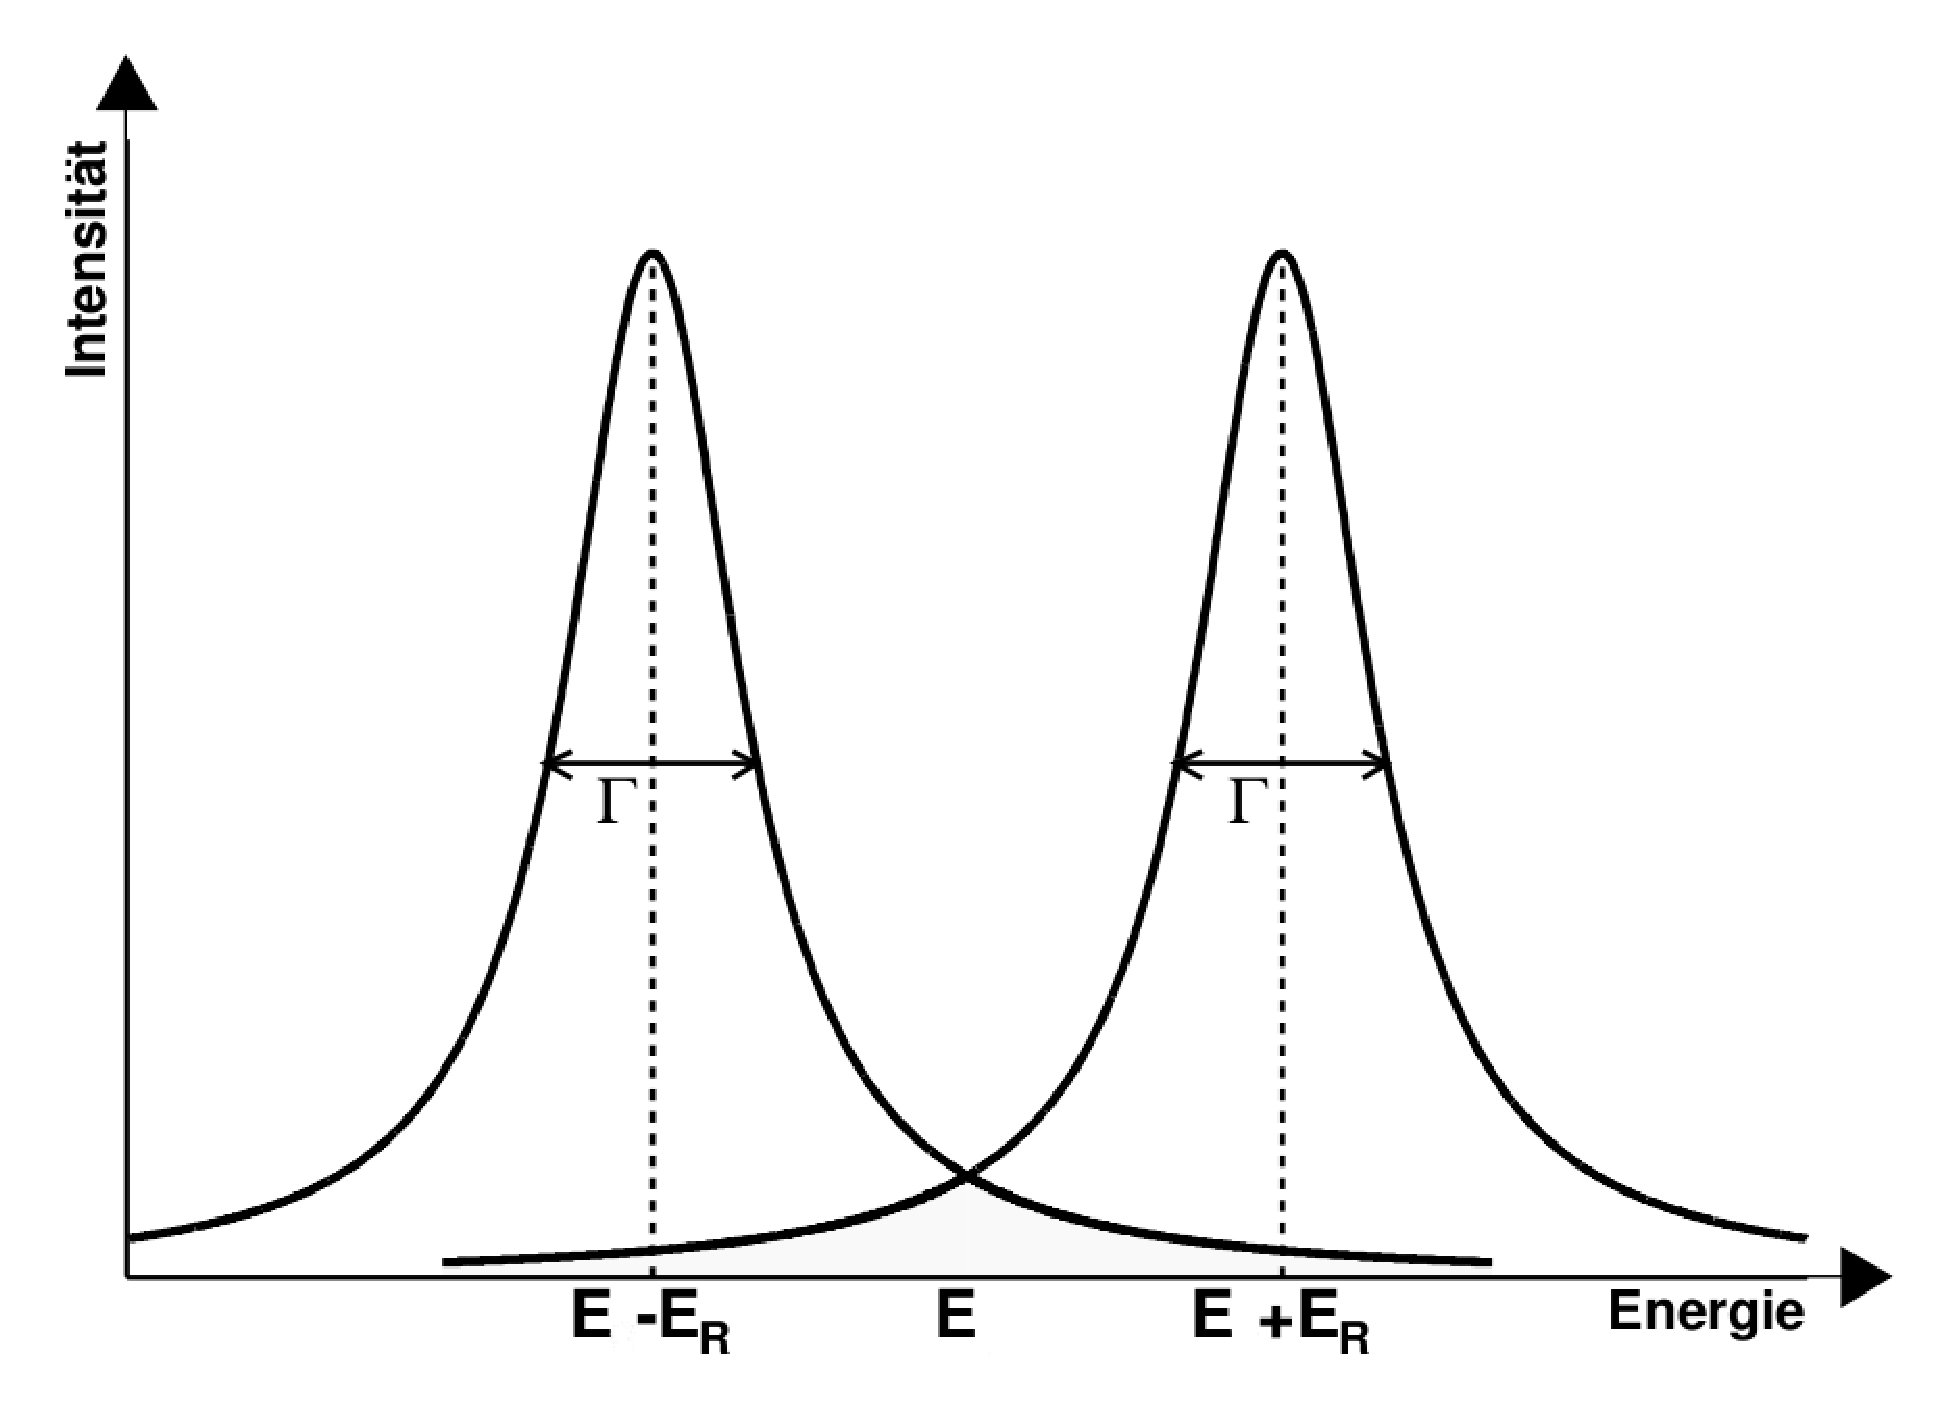
\includegraphics[width=0.9\linewidth]{pictures/energieverschiebung.eps}
 \caption{Energieverschiebung von Emissions- und Absorptionslinie}
 \label{energieverschiebung}
\end{figure}
Bei Übergängen an Atomen im Sichtbaren Bereich ist die Linienbreite, aufgrund der relativ kleinen Übergangsenergie (eV-Bereich) gegenüber der Atommasse,
groß gegenüber der Verschiebung der beiden Linien. Kommt zur natürlichen Linienbreite auch noch die Dopplerverbreiterung wenn sich die Atome ein einem Gas
befinden so kann fast vollständige Überlappung der beiden Linien erreicht werden. Es kommt also fast immer zu Resonanzabsorption.

Bei Kernübergängen im $\gamma$-Bereich ist die Übergangsenergie im keV-Bereich und somit groß gegen die Masse des Kerns. Die beiden Linien überschneiden sich
selbst mit Dopplerverbreiterung garnicht oder fast garnicht. In einem solchen System wird also keine Resonanzabsorption zu beobachten sein zumindest nicht
wenn man das System nicht dahingehend beeinflussen kann dass die Linien näher zusammenrücken. Hier kommt der Mößbauereffekt gelegen.

\subsection{Mößbauereffekt}
Rudolf Mößbauer entdeckte, dass wenn man die Kerne nicht frei vorliegen hat sondern in ein Gitter bindet, kann man erreichen das der Rückstoßimpuls $\vec{p}_g$
auf den gesamten Kristall übertragen wird. Wegen der riesigen Masse des Kristalls ist nach Gleichung \ref{e_r} damit aber, solange keine Gitterschwingungen (Phononen) angeregt werden,
fast kein Energieübertrag verbunden. Die Emissions- und Absorptionslinie sind somit nicht gegeneinander verschoben und es kann Resonanzabsorption auftreten. Die sogenannte
``rückstoßfreie Resonanzabsorption''.

\subsection{Isomerieverschiebung}
\subsection{Hyperfeinstrukturaufspaltung}
\subsection{Linienverbreiterung}

\section{Versuchsaufbau}

\section{Durchführung}

\section{Auswertung}

\section{Zusammenfassung}

\section{Zusatz: Geschwindigkeitsmessung}
Nach Aussagen des Assistenten stellte sich bei diesem Versuchsaufbau schon seit längerem die Frage wie groß der Fehler der Geschindigkeit des Schlittens also des Absorbers ist. Somit haben wir uns ein paar Gedanken gemacht wie man denn die Geschwindikeit des Schlittens Messen kann. Eine Zeitmessung über lange Strecken macht keinen Sinn, da die Konstanz der Geschindigkeit untersucht werden soll. Wir hatten die Idee den Sensor einer optischen Maus zu verwenden: 800 dpi, sollten eine ausreichende Genauigkeit bringen.

Gängige Maussensoren haben zwei mögliche Ausgänge: Ein serieller Ausgang und eine ``Quadratur Ausgang'' also 2 Pins für jede Achse, wobei die Zustände im Ring je nach Bewegungsrichtung linksrum oder rechtsrum aufeinander folgen.

Wir entschienden uns mit der Intention die kleinstmöglichen Inkremente zu erhalten für den letzeren Anschluss und nahmen einen Microcontroller für die Auswertung der Bewegung. Anfangs war das ein Microchip PIC18F4550, da dieser jedoch Probleme machte stiegen wir auf einen Atmel ATMega32 um. Leider mussten wir feststellen als wir die ersten Geschwindigkeitshistogramme betrachteten, dass ein Fehler vorlag. Es stellte sich heraus das der 16MHz Takt des Microcontrollers nicht ausreichte um alle Zustandsänderungen des Maussensors zu erfassen. Bei schnellen Bewegungen kam der Chip nicht nach einem Interrupt nicht mehr in den normalen Programmablauf da schon der nächste Interrupt ausgelöst war.


Also musste doch die 1te Anschlussmethode herhalten, diesmal aber ohne Microcontroller und stattdessen direkt am PC angeschlossen.
\end{document}
